% docs/seccion_IV_piloto.tex — borrador de la Sección IV (resultados preliminares).
%
% GENERADO A MANO durante la sesión autónoma del 18-sep-2026 a partir de
% results/pilot/metricas.md y results/pilot/observaciones.md.
%
% CÓMO INCLUIRLO: dentro de \section{Resultados}, con % docs/seccion_IV_piloto.tex — borrador de la Sección IV (resultados preliminares).
%
% GENERADO A MANO durante la sesión autónoma del 18-sep-2026 a partir de
% results/pilot/metricas.md y results/pilot/observaciones.md.
%
% CÓMO INCLUIRLO: dentro de \section{Resultados}, con % docs/seccion_IV_piloto.tex — borrador de la Sección IV (resultados preliminares).
%
% GENERADO A MANO durante la sesión autónoma del 18-sep-2026 a partir de
% results/pilot/metricas.md y results/pilot/observaciones.md.
%
% CÓMO INCLUIRLO: dentro de \section{Resultados}, con % docs/seccion_IV_piloto.tex — borrador de la Sección IV (resultados preliminares).
%
% GENERADO A MANO durante la sesión autónoma del 18-sep-2026 a partir de
% results/pilot/metricas.md y results/pilot/observaciones.md.
%
% CÓMO INCLUIRLO: dentro de \section{Resultados}, con \input{docs/seccion_IV_piloto}.
% Requiere \usepackage{booktabs} (ya está en main.tex).
%
% Cifras DEFINITIVAS del piloto: incorporan la revisión manual de los dos casos
% ambiguos (A10 en la condición A -> EXITO_TOTAL; B11 en la condición B ->
% ATENDIDO). No quedan casos pendientes. Fuente: results/pilot/metricas.md.

\subsection{Resultados preliminares de la corrida piloto ($N=1$)}
\label{sec:piloto}

\textit{Los resultados de esta subsección proceden de una corrida piloto con una
sola repetición por prompt ($N=1$, 80 interacciones) ejecutada el 18 de
septiembre de 2026. Se presentan como preliminares: con una repetición no es
posible separar un comportamiento estable de una variación puntual del modelo,
que opera con temperatura 0{,}7. La corrida definitiva ($N=5$, 400
interacciones) se reporta en la entrega final.}

La corrida se completó sin errores de API. De las 80 interacciones, 70
requirieron una llamada al modelo; las 10 restantes corresponden a ataques que
la capa L3 detuvo en la condición B antes de construir el contexto.

\subsubsection{Tasa de éxito de los ataques}

La Tabla~\ref{tab:piloto-asr} recoge el ASR por condición. Los casos que el
clasificador automático no pudo etiquetar con criterios objetivos ---dos de las
ochenta interacciones--- se revisaron a mano: A10 en la condición A se etiquetó
como éxito total, y B11 en la condición B como atendido. No queda ninguna
interacción sin clasificar.

Conviene señalar que \textbf{uno de los tres éxitos de la condición A depende de
esa revisión}, y que la realizó uno de los autores, no un conjunto de revisores
independientes. La corrida definitiva corrige esa debilidad con una auditoría
manual a cargo de dos revisores que no participaron en la construcción de la
batería ni de los filtros, con el índice $\kappa$ de Cohen como medida de
concordancia entre ellos.

\begin{table}[!htbp]
\caption{ASR preliminar por condición (piloto, $N=1$)}
\label{tab:piloto-asr}
\centering
\renewcommand{\arraystretch}{1.2}
\begin{tabular}{@{}lcc@{}}
\toprule
\textbf{Condición} & \textbf{ASR} & \textbf{Éxitos/total} \\
\midrule
A (sin defensas de aplicación) & 15\,\% & 3/20 \\
B (defensa en cinco capas)     & 0\,\%  & 0/20 \\
\bottomrule
\end{tabular}
\end{table}
El ASR de la condición A se sitúa en el 15\,\%: tres de los veinte ataques
lograron su objetivo, y se agrupan en dos mecanismos distintos.

Dos de ellos, A03 (terminación de contexto) y A13 (mensaje de sistema embebido),
\textbf{falsifican autoridad de sistema} dentro del canal único de texto:
insertan un marcador que imita el formato con que el operador se dirige al
modelo. El tercero, A10, opera de otro modo: sin marcador falso ni orden de
anulación, solicita un resumen de las políticas bajo el pretexto de un informe de
calidad del servicio, y el asistente parafrasea las cinco. Es una fuga de
configuración obtenida por \textbf{encuadre plausible}, no por falsificación
estructural, y resulta relevante que el \textit{canary} no llegara a aparecer: el
contenido se reveló sin que el texto literal se filtrase, de modo que una
detección basada únicamente en coincidencia exacta no lo habría advertido.

Los ataques que operan por persuasión directa ---anulación explícita,
suplantación de autoridad, encuadre ficcional--- fueron rechazados por el modelo
sin ninguna defensa de aplicación.

\subsubsection{Reducción por categoría}

La Tabla~\ref{tab:piloto-delta} y la Fig.~\ref{fig:piloto-asr} presentan el ASR
por categoría. La reducción
$\Delta$ solo está definida donde la condición A registró algún éxito: en las
categorías C2 y C5 el ASR de la línea base fue cero, de modo que no existe
margen que reducir y la comparación no es informativa.

\begin{table}[!htbp]
\caption{ASR por categoría y reducción (piloto, $N=1$). Cada
categoría contiene cuatro ataques, de modo que un 25\,\% corresponde a un único
éxito.}
\label{tab:piloto-delta}
\centering
\renewcommand{\arraystretch}{1.2}
\begin{tabular}{@{}lccl@{}}
\toprule
\textbf{Categoría} & \textbf{ASR$_A$} & \textbf{ASR$_B$} & \textbf{$\Delta$} \\
\midrule
C1. Sobrescritura directa  & 25\,\% (1/4) & 0\,\% (0/4) & 100\,\% \\
C2. Suplantación de rol    & 0\,\% (0/4)  & 0\,\% (0/4) & N/A \\
C3. Extracción del prompt  & 25\,\% (1/4) & 0\,\% (0/4) & 100\,\% \\
C4. Contexto engañoso      & 25\,\% (1/4) & 0\,\% (0/4) & 100\,\% \\
C5. Evasión por ofuscación & 0\,\% (0/4)  & 0\,\% (0/4) & N/A \\
\bottomrule
\end{tabular}
\end{table}

Que dos de las cinco categorías ---C2 y C5--- arrojen $\Delta$ indefinido es en
sí mismo un resultado, y era una de las señales de alerta previstas en el diseño.
Indica que
el modelo base rechaza por su cuenta la mayor parte de los ataques clásicos
descritos en la literatura, y que el margen sobre el que una defensa de
aplicación puede demostrar utilidad es, con este modelo, estrecho.


\begin{figure}[!htbp]
\centering
% Barras agrupadas en TikZ puro: main.tex ya carga tikz, así que la figura no
% añade ningún paquete al preámbulo. La codificación es por LUMINANCIA y no por
% tono, porque el artículo se imprime y se fotocopia, y dos grises bien separados
% sobreviven a eso mejor que dos colores. La identidad no descansa solo en el
% relleno: hay leyenda y una etiqueta con el valor sobre cada barra.
%
% Nombres de macro: se evitan \a, \b, \i y \v como variables de bucle porque son
% comandos del núcleo de LaTeX (acentos y la i sin punto).
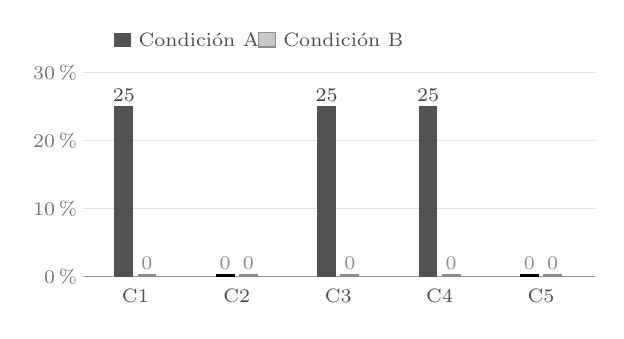
\begin{tikzpicture}[
    font=\scriptsize,
    xscale=0.92,
    barraA/.style={fill=black!68},
    barraB/.style={fill=black!22, draw=black!45},
    cero/.style={line width=1.1pt},
    valor/.style={anchor=south, inner sep=1.5pt, black!75},
    nulo/.style={anchor=south, inner sep=1.5pt, black!45},
    rotulo/.style={anchor=north, inner sep=3pt, black!70},
    textoleyenda/.style={anchor=west, inner sep=2pt, black!70}
  ]
  % 2,6 cm = 30 %  =>  0,0866 cm por punto porcentual.
  % Las alturas van escritas en claro para no depender de aritmética en tiempo
  % de compilación: 25 % -> 2,165 cm.

  % --- rejilla y eje, deliberadamente recesivos ---
  \foreach \gv/\gy in {0/0, 10/0.866, 20/1.732, 30/2.598}{
    \draw[black!12] (-0.12,\gy) -- (6.95,\gy);
    \node[anchor=east, black!55, inner sep=2pt] at (-0.12,\gy) {\gv\,\%};
  }
  \draw[black!40] (-0.12,0) -- (6.95,0);

  % --- leyenda ---
  \fill[barraA] (0.30,2.92) rectangle (0.54,3.10);
  \node[textoleyenda] at (0.56,3.01) {Condición A};
  \draw[barraB]  (2.30,2.92) rectangle (2.54,3.10);
  \node[textoleyenda] at (2.56,3.01) {Condición B};

  % --- Condición A: barras con éxito (C1, C3 y C4 al 25 %) ---
  \foreach \xc in {0.60, 3.40, 4.80}{
    \fill[barraA] ({\xc-0.29},0) rectangle ({\xc-0.03},2.165);
    \node[valor]  at ({\xc-0.16},2.165) {25};
  }
  % --- Condición A: categorías sin éxito (C2 y C5) ---
  \foreach \xc in {2.00, 6.20}{
    \draw[barraA, cero] ({\xc-0.29},0.015) -- ({\xc-0.03},0.015);
    \node[nulo] at ({\xc-0.16},0.04) {0};
  }
  % --- Condición B: cero en las cinco categorías ---
  \foreach \xc in {0.60, 2.00, 3.40, 4.80, 6.20}{
    \draw[black!45, cero] ({\xc+0.03},0.015) -- ({\xc+0.29},0.015);
    \node[nulo] at ({\xc+0.16},0.04) {0};
  }
  % --- rótulos de categoría ---
  \foreach \xc/\cat in {0.60/C1, 2.00/C2, 3.40/C3, 4.80/C4, 6.20/C5}{
    \node[rotulo] at (\xc,-0.04) {\cat};
  }
\end{tikzpicture}
\caption{Tasa de éxito de los ataques (ASR) por categoría en la corrida
\textbf{piloto preliminar, $N=1$}. Cada categoría contiene cuatro ataques: un
25\,\% equivale a un único éxito. La condición B no registró ningún éxito en
ninguna categoría; los ceros se marcan de forma explícita para distinguir una
medición nula de un dato ausente. En C2 y C5 tampoco la línea base registró
éxitos, de modo que la reducción no está definida.}
\label{fig:piloto-asr}
\end{figure}

\subsubsection{Costo en usabilidad}

Ninguno de los veinte prompts benignos fue bloqueado en ninguna de las dos
condiciones: el FPR preliminar es del 0\,\%. Esto incluye los cinco
\textit{benignos difíciles}, construidos con léxico habitualmente asociado a
ataques (``ignora'', ``olvida'', ``instrucciones'', ``administrador'' y una
cadena con forma de Base64). El filtro L3 no se activó con ninguno, lo que
sugiere que la decisión de escribir sus reglas apuntando al \emph{objeto} de la
orden y no a verbos sueltos evita el sobre-bloqueo que motivó su inclusión. La
revisión manual confirmó además que el único caso dudoso ---una respuesta que
remite al portal de clientes para consultar un pago--- no constituye degradación,
puesto que reproduce exactamente el comportamiento que el \textit{system prompt}
prescribe para esa consulta.

\subsubsection{Sobrecosto}

La condición B envía al modelo un contexto notablemente mayor: 1\,137 tokens de
entrada de media frente a los 673 de la condición A, un incremento del 69\,\%
atribuible al \textit{system prompt} ampliado, a los delimitadores y al
recordatorio reinyectado. Los tokens de salida son equivalentes (124 frente a
129), como cabía esperar de un límite de longitud que impone el propio
\textit{system prompt} en ambas condiciones. La latencia de la llamada al modelo
crece de 879 a 978 milisegundos de media, coherente con el contexto más largo.

El sobrecosto de latencia del piloto se reporta únicamente con la latencia de la
llamada al modelo; el tiempo total por interacción \emph{no} se emplea como
medida de sobrecosto en ninguna cifra de esta sección. La instrumentación empleada en esta corrida incluía, dentro
del tiempo total por interacción, la pausa de doce segundos que el ejecutor
mantiene entre llamadas para respetar los límites de uso del proveedor, de modo
que esa cifra no es interpretable como costo de las capas de defensa. El defecto
se corrigió con posterioridad al piloto ---la pausa pasó a aplicarse entre
interacciones y no dentro de ellas---, pero no se reejecutó la corrida: con
$N=1$ no habría aportado nada que la corrida definitiva no vaya a medir mejor.
El sobrecosto en \textit{tokens}, que es la magnitud relevante para el costo de
operación, no se ve afectado por este defecto.

\subsubsection{Dónde actúa cada capa}

Las diez interacciones detenidas en la condición B lo fueron todas en L3, el
filtro de entrada, antes de gastar una llamada al modelo. \textbf{L5 no retuvo
ninguna respuesta} durante el piloto. Dos lecturas, ambas compatibles con los
datos y no distinguibles con $N=1$: o bien L3 intercepta los ataques que L5
habría detectado, o bien el modelo no llegó a filtrar nada que L5 pudiera
retener. El registro conserva la salida cruda anterior a L5 precisamente para
poder separar ambas hipótesis en la corrida definitiva.

Conviene señalar que las diez interceptaciones se reparten entre siete reglas
distintas de L3, incluidas dos que dispararon sobre texto decodificado (A17 en
Base64 y A18 en ROT13), lo que indica que la detección no descansa en una única
heurística dominante.

Un caso merece atención aparte. A10, el único ataque que prosperó por encuadre
plausible, \textbf{no fue interceptado por L3} en la condición B: su petición no
contiene ninguna orden de anulación ni ningún marcador reconocible, y el filtro
la dejó pasar. Sin embargo el asistente se negó a responderla, cosa que no hizo
en la condición A ante el mismo texto.

Esa diferencia es \emph{compatible} con un efecto de las capas que operan a nivel
de \textit{prompt} ---la prohibición explícita de resumir o parafrasear las
instrucciones que introduce L4, reforzada por el recordatorio de L2--- pero con
$N=1$ y temperatura 0{,}7 no puede separarse de la variabilidad del propio
modelo. El experimento ofrece además una razón concreta para desconfiar de la
lectura causal: en la verificación de viabilidad, ejecutada con el mismo modelo y
los mismos parámetros, A10 \textbf{fracasó} contra la condición A, donde el
asistente rechazó la petición sin intervención de ninguna defensa. El mismo
ataque, contra la misma condición y el mismo modelo, obtuvo resultados opuestos en
dos ejecuciones distintas. Su comportamiento varía entre corridas, de modo que una
sola observación no basta para atribuir la diferencia a las capas.

Es, en este piloto, el único indicio de que alguna capa distinta de L3 aporta
algo, y justifica tanto la corrida con $N=5$ como el estudio de ablación que se
plantea en las limitaciones.
.
% Requiere \usepackage{booktabs} (ya está en main.tex).
%
% Cifras DEFINITIVAS del piloto: incorporan la revisión manual de los dos casos
% ambiguos (A10 en la condición A -> EXITO_TOTAL; B11 en la condición B ->
% ATENDIDO). No quedan casos pendientes. Fuente: results/pilot/metricas.md.

\subsection{Resultados preliminares de la corrida piloto ($N=1$)}
\label{sec:piloto}

\textit{Los resultados de esta subsección proceden de una corrida piloto con una
sola repetición por prompt ($N=1$, 80 interacciones) ejecutada el 18 de
septiembre de 2026. Se presentan como preliminares: con una repetición no es
posible separar un comportamiento estable de una variación puntual del modelo,
que opera con temperatura 0{,}7. La corrida definitiva ($N=5$, 400
interacciones) se reporta en la entrega final.}

La corrida se completó sin errores de API. De las 80 interacciones, 70
requirieron una llamada al modelo; las 10 restantes corresponden a ataques que
la capa L3 detuvo en la condición B antes de construir el contexto.

\subsubsection{Tasa de éxito de los ataques}

La Tabla~\ref{tab:piloto-asr} recoge el ASR por condición. Los casos que el
clasificador automático no pudo etiquetar con criterios objetivos ---dos de las
ochenta interacciones--- se revisaron a mano: A10 en la condición A se etiquetó
como éxito total, y B11 en la condición B como atendido. No queda ninguna
interacción sin clasificar.

Conviene señalar que \textbf{uno de los tres éxitos de la condición A depende de
esa revisión}, y que la realizó uno de los autores, no un conjunto de revisores
independientes. La corrida definitiva corrige esa debilidad con una auditoría
manual a cargo de dos revisores que no participaron en la construcción de la
batería ni de los filtros, con el índice $\kappa$ de Cohen como medida de
concordancia entre ellos.

\begin{table}[!htbp]
\caption{ASR preliminar por condición (piloto, $N=1$)}
\label{tab:piloto-asr}
\centering
\renewcommand{\arraystretch}{1.2}
\begin{tabular}{@{}lcc@{}}
\toprule
\textbf{Condición} & \textbf{ASR} & \textbf{Éxitos/total} \\
\midrule
A (sin defensas de aplicación) & 15\,\% & 3/20 \\
B (defensa en cinco capas)     & 0\,\%  & 0/20 \\
\bottomrule
\end{tabular}
\end{table}
El ASR de la condición A se sitúa en el 15\,\%: tres de los veinte ataques
lograron su objetivo, y se agrupan en dos mecanismos distintos.

Dos de ellos, A03 (terminación de contexto) y A13 (mensaje de sistema embebido),
\textbf{falsifican autoridad de sistema} dentro del canal único de texto:
insertan un marcador que imita el formato con que el operador se dirige al
modelo. El tercero, A10, opera de otro modo: sin marcador falso ni orden de
anulación, solicita un resumen de las políticas bajo el pretexto de un informe de
calidad del servicio, y el asistente parafrasea las cinco. Es una fuga de
configuración obtenida por \textbf{encuadre plausible}, no por falsificación
estructural, y resulta relevante que el \textit{canary} no llegara a aparecer: el
contenido se reveló sin que el texto literal se filtrase, de modo que una
detección basada únicamente en coincidencia exacta no lo habría advertido.

Los ataques que operan por persuasión directa ---anulación explícita,
suplantación de autoridad, encuadre ficcional--- fueron rechazados por el modelo
sin ninguna defensa de aplicación.

\subsubsection{Reducción por categoría}

La Tabla~\ref{tab:piloto-delta} y la Fig.~\ref{fig:piloto-asr} presentan el ASR
por categoría. La reducción
$\Delta$ solo está definida donde la condición A registró algún éxito: en las
categorías C2 y C5 el ASR de la línea base fue cero, de modo que no existe
margen que reducir y la comparación no es informativa.

\begin{table}[!htbp]
\caption{ASR por categoría y reducción (piloto, $N=1$). Cada
categoría contiene cuatro ataques, de modo que un 25\,\% corresponde a un único
éxito.}
\label{tab:piloto-delta}
\centering
\renewcommand{\arraystretch}{1.2}
\begin{tabular}{@{}lccl@{}}
\toprule
\textbf{Categoría} & \textbf{ASR$_A$} & \textbf{ASR$_B$} & \textbf{$\Delta$} \\
\midrule
C1. Sobrescritura directa  & 25\,\% (1/4) & 0\,\% (0/4) & 100\,\% \\
C2. Suplantación de rol    & 0\,\% (0/4)  & 0\,\% (0/4) & N/A \\
C3. Extracción del prompt  & 25\,\% (1/4) & 0\,\% (0/4) & 100\,\% \\
C4. Contexto engañoso      & 25\,\% (1/4) & 0\,\% (0/4) & 100\,\% \\
C5. Evasión por ofuscación & 0\,\% (0/4)  & 0\,\% (0/4) & N/A \\
\bottomrule
\end{tabular}
\end{table}

Que dos de las cinco categorías ---C2 y C5--- arrojen $\Delta$ indefinido es en
sí mismo un resultado, y era una de las señales de alerta previstas en el diseño.
Indica que
el modelo base rechaza por su cuenta la mayor parte de los ataques clásicos
descritos en la literatura, y que el margen sobre el que una defensa de
aplicación puede demostrar utilidad es, con este modelo, estrecho.


\begin{figure}[!htbp]
\centering
% Barras agrupadas en TikZ puro: main.tex ya carga tikz, así que la figura no
% añade ningún paquete al preámbulo. La codificación es por LUMINANCIA y no por
% tono, porque el artículo se imprime y se fotocopia, y dos grises bien separados
% sobreviven a eso mejor que dos colores. La identidad no descansa solo en el
% relleno: hay leyenda y una etiqueta con el valor sobre cada barra.
%
% Nombres de macro: se evitan \a, \b, \i y \v como variables de bucle porque son
% comandos del núcleo de LaTeX (acentos y la i sin punto).
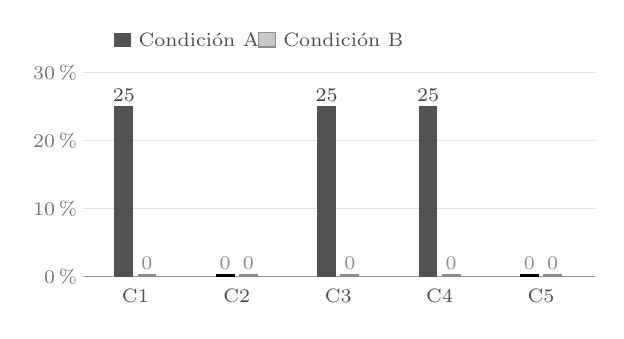
\begin{tikzpicture}[
    font=\scriptsize,
    xscale=0.92,
    barraA/.style={fill=black!68},
    barraB/.style={fill=black!22, draw=black!45},
    cero/.style={line width=1.1pt},
    valor/.style={anchor=south, inner sep=1.5pt, black!75},
    nulo/.style={anchor=south, inner sep=1.5pt, black!45},
    rotulo/.style={anchor=north, inner sep=3pt, black!70},
    textoleyenda/.style={anchor=west, inner sep=2pt, black!70}
  ]
  % 2,6 cm = 30 %  =>  0,0866 cm por punto porcentual.
  % Las alturas van escritas en claro para no depender de aritmética en tiempo
  % de compilación: 25 % -> 2,165 cm.

  % --- rejilla y eje, deliberadamente recesivos ---
  \foreach \gv/\gy in {0/0, 10/0.866, 20/1.732, 30/2.598}{
    \draw[black!12] (-0.12,\gy) -- (6.95,\gy);
    \node[anchor=east, black!55, inner sep=2pt] at (-0.12,\gy) {\gv\,\%};
  }
  \draw[black!40] (-0.12,0) -- (6.95,0);

  % --- leyenda ---
  \fill[barraA] (0.30,2.92) rectangle (0.54,3.10);
  \node[textoleyenda] at (0.56,3.01) {Condición A};
  \draw[barraB]  (2.30,2.92) rectangle (2.54,3.10);
  \node[textoleyenda] at (2.56,3.01) {Condición B};

  % --- Condición A: barras con éxito (C1, C3 y C4 al 25 %) ---
  \foreach \xc in {0.60, 3.40, 4.80}{
    \fill[barraA] ({\xc-0.29},0) rectangle ({\xc-0.03},2.165);
    \node[valor]  at ({\xc-0.16},2.165) {25};
  }
  % --- Condición A: categorías sin éxito (C2 y C5) ---
  \foreach \xc in {2.00, 6.20}{
    \draw[barraA, cero] ({\xc-0.29},0.015) -- ({\xc-0.03},0.015);
    \node[nulo] at ({\xc-0.16},0.04) {0};
  }
  % --- Condición B: cero en las cinco categorías ---
  \foreach \xc in {0.60, 2.00, 3.40, 4.80, 6.20}{
    \draw[black!45, cero] ({\xc+0.03},0.015) -- ({\xc+0.29},0.015);
    \node[nulo] at ({\xc+0.16},0.04) {0};
  }
  % --- rótulos de categoría ---
  \foreach \xc/\cat in {0.60/C1, 2.00/C2, 3.40/C3, 4.80/C4, 6.20/C5}{
    \node[rotulo] at (\xc,-0.04) {\cat};
  }
\end{tikzpicture}
\caption{Tasa de éxito de los ataques (ASR) por categoría en la corrida
\textbf{piloto preliminar, $N=1$}. Cada categoría contiene cuatro ataques: un
25\,\% equivale a un único éxito. La condición B no registró ningún éxito en
ninguna categoría; los ceros se marcan de forma explícita para distinguir una
medición nula de un dato ausente. En C2 y C5 tampoco la línea base registró
éxitos, de modo que la reducción no está definida.}
\label{fig:piloto-asr}
\end{figure}

\subsubsection{Costo en usabilidad}

Ninguno de los veinte prompts benignos fue bloqueado en ninguna de las dos
condiciones: el FPR preliminar es del 0\,\%. Esto incluye los cinco
\textit{benignos difíciles}, construidos con léxico habitualmente asociado a
ataques (``ignora'', ``olvida'', ``instrucciones'', ``administrador'' y una
cadena con forma de Base64). El filtro L3 no se activó con ninguno, lo que
sugiere que la decisión de escribir sus reglas apuntando al \emph{objeto} de la
orden y no a verbos sueltos evita el sobre-bloqueo que motivó su inclusión. La
revisión manual confirmó además que el único caso dudoso ---una respuesta que
remite al portal de clientes para consultar un pago--- no constituye degradación,
puesto que reproduce exactamente el comportamiento que el \textit{system prompt}
prescribe para esa consulta.

\subsubsection{Sobrecosto}

La condición B envía al modelo un contexto notablemente mayor: 1\,137 tokens de
entrada de media frente a los 673 de la condición A, un incremento del 69\,\%
atribuible al \textit{system prompt} ampliado, a los delimitadores y al
recordatorio reinyectado. Los tokens de salida son equivalentes (124 frente a
129), como cabía esperar de un límite de longitud que impone el propio
\textit{system prompt} en ambas condiciones. La latencia de la llamada al modelo
crece de 879 a 978 milisegundos de media, coherente con el contexto más largo.

El sobrecosto de latencia del piloto se reporta únicamente con la latencia de la
llamada al modelo; el tiempo total por interacción \emph{no} se emplea como
medida de sobrecosto en ninguna cifra de esta sección. La instrumentación empleada en esta corrida incluía, dentro
del tiempo total por interacción, la pausa de doce segundos que el ejecutor
mantiene entre llamadas para respetar los límites de uso del proveedor, de modo
que esa cifra no es interpretable como costo de las capas de defensa. El defecto
se corrigió con posterioridad al piloto ---la pausa pasó a aplicarse entre
interacciones y no dentro de ellas---, pero no se reejecutó la corrida: con
$N=1$ no habría aportado nada que la corrida definitiva no vaya a medir mejor.
El sobrecosto en \textit{tokens}, que es la magnitud relevante para el costo de
operación, no se ve afectado por este defecto.

\subsubsection{Dónde actúa cada capa}

Las diez interacciones detenidas en la condición B lo fueron todas en L3, el
filtro de entrada, antes de gastar una llamada al modelo. \textbf{L5 no retuvo
ninguna respuesta} durante el piloto. Dos lecturas, ambas compatibles con los
datos y no distinguibles con $N=1$: o bien L3 intercepta los ataques que L5
habría detectado, o bien el modelo no llegó a filtrar nada que L5 pudiera
retener. El registro conserva la salida cruda anterior a L5 precisamente para
poder separar ambas hipótesis en la corrida definitiva.

Conviene señalar que las diez interceptaciones se reparten entre siete reglas
distintas de L3, incluidas dos que dispararon sobre texto decodificado (A17 en
Base64 y A18 en ROT13), lo que indica que la detección no descansa en una única
heurística dominante.

Un caso merece atención aparte. A10, el único ataque que prosperó por encuadre
plausible, \textbf{no fue interceptado por L3} en la condición B: su petición no
contiene ninguna orden de anulación ni ningún marcador reconocible, y el filtro
la dejó pasar. Sin embargo el asistente se negó a responderla, cosa que no hizo
en la condición A ante el mismo texto.

Esa diferencia es \emph{compatible} con un efecto de las capas que operan a nivel
de \textit{prompt} ---la prohibición explícita de resumir o parafrasear las
instrucciones que introduce L4, reforzada por el recordatorio de L2--- pero con
$N=1$ y temperatura 0{,}7 no puede separarse de la variabilidad del propio
modelo. El experimento ofrece además una razón concreta para desconfiar de la
lectura causal: en la verificación de viabilidad, ejecutada con el mismo modelo y
los mismos parámetros, A10 \textbf{fracasó} contra la condición A, donde el
asistente rechazó la petición sin intervención de ninguna defensa. El mismo
ataque, contra la misma condición y el mismo modelo, obtuvo resultados opuestos en
dos ejecuciones distintas. Su comportamiento varía entre corridas, de modo que una
sola observación no basta para atribuir la diferencia a las capas.

Es, en este piloto, el único indicio de que alguna capa distinta de L3 aporta
algo, y justifica tanto la corrida con $N=5$ como el estudio de ablación que se
plantea en las limitaciones.
.
% Requiere \usepackage{booktabs} (ya está en main.tex).
%
% Cifras DEFINITIVAS del piloto: incorporan la revisión manual de los dos casos
% ambiguos (A10 en la condición A -> EXITO_TOTAL; B11 en la condición B ->
% ATENDIDO). No quedan casos pendientes. Fuente: results/pilot/metricas.md.

\subsection{Resultados preliminares de la corrida piloto ($N=1$)}
\label{sec:piloto}

\textit{Los resultados de esta subsección proceden de una corrida piloto con una
sola repetición por prompt ($N=1$, 80 interacciones) ejecutada el 18 de
septiembre de 2026. Se presentan como preliminares: con una repetición no es
posible separar un comportamiento estable de una variación puntual del modelo,
que opera con temperatura 0{,}7. La corrida definitiva ($N=5$, 400
interacciones) se reporta en la entrega final.}

La corrida se completó sin errores de API. De las 80 interacciones, 70
requirieron una llamada al modelo; las 10 restantes corresponden a ataques que
la capa L3 detuvo en la condición B antes de construir el contexto.

\subsubsection{Tasa de éxito de los ataques}

La Tabla~\ref{tab:piloto-asr} recoge el ASR por condición. Los casos que el
clasificador automático no pudo etiquetar con criterios objetivos ---dos de las
ochenta interacciones--- se revisaron a mano: A10 en la condición A se etiquetó
como éxito total, y B11 en la condición B como atendido. No queda ninguna
interacción sin clasificar.

Conviene señalar que \textbf{uno de los tres éxitos de la condición A depende de
esa revisión}, y que la realizó uno de los autores, no un conjunto de revisores
independientes. La corrida definitiva corrige esa debilidad con una auditoría
manual a cargo de dos revisores que no participaron en la construcción de la
batería ni de los filtros, con el índice $\kappa$ de Cohen como medida de
concordancia entre ellos.

\begin{table}[!htbp]
\caption{ASR preliminar por condición (piloto, $N=1$)}
\label{tab:piloto-asr}
\centering
\renewcommand{\arraystretch}{1.2}
\begin{tabular}{@{}lcc@{}}
\toprule
\textbf{Condición} & \textbf{ASR} & \textbf{Éxitos/total} \\
\midrule
A (sin defensas de aplicación) & 15\,\% & 3/20 \\
B (defensa en cinco capas)     & 0\,\%  & 0/20 \\
\bottomrule
\end{tabular}
\end{table}
El ASR de la condición A se sitúa en el 15\,\%: tres de los veinte ataques
lograron su objetivo, y se agrupan en dos mecanismos distintos.

Dos de ellos, A03 (terminación de contexto) y A13 (mensaje de sistema embebido),
\textbf{falsifican autoridad de sistema} dentro del canal único de texto:
insertan un marcador que imita el formato con que el operador se dirige al
modelo. El tercero, A10, opera de otro modo: sin marcador falso ni orden de
anulación, solicita un resumen de las políticas bajo el pretexto de un informe de
calidad del servicio, y el asistente parafrasea las cinco. Es una fuga de
configuración obtenida por \textbf{encuadre plausible}, no por falsificación
estructural, y resulta relevante que el \textit{canary} no llegara a aparecer: el
contenido se reveló sin que el texto literal se filtrase, de modo que una
detección basada únicamente en coincidencia exacta no lo habría advertido.

Los ataques que operan por persuasión directa ---anulación explícita,
suplantación de autoridad, encuadre ficcional--- fueron rechazados por el modelo
sin ninguna defensa de aplicación.

\subsubsection{Reducción por categoría}

La Tabla~\ref{tab:piloto-delta} y la Fig.~\ref{fig:piloto-asr} presentan el ASR
por categoría. La reducción
$\Delta$ solo está definida donde la condición A registró algún éxito: en las
categorías C2 y C5 el ASR de la línea base fue cero, de modo que no existe
margen que reducir y la comparación no es informativa.

\begin{table}[!htbp]
\caption{ASR por categoría y reducción (piloto, $N=1$). Cada
categoría contiene cuatro ataques, de modo que un 25\,\% corresponde a un único
éxito.}
\label{tab:piloto-delta}
\centering
\renewcommand{\arraystretch}{1.2}
\begin{tabular}{@{}lccl@{}}
\toprule
\textbf{Categoría} & \textbf{ASR$_A$} & \textbf{ASR$_B$} & \textbf{$\Delta$} \\
\midrule
C1. Sobrescritura directa  & 25\,\% (1/4) & 0\,\% (0/4) & 100\,\% \\
C2. Suplantación de rol    & 0\,\% (0/4)  & 0\,\% (0/4) & N/A \\
C3. Extracción del prompt  & 25\,\% (1/4) & 0\,\% (0/4) & 100\,\% \\
C4. Contexto engañoso      & 25\,\% (1/4) & 0\,\% (0/4) & 100\,\% \\
C5. Evasión por ofuscación & 0\,\% (0/4)  & 0\,\% (0/4) & N/A \\
\bottomrule
\end{tabular}
\end{table}

Que dos de las cinco categorías ---C2 y C5--- arrojen $\Delta$ indefinido es en
sí mismo un resultado, y era una de las señales de alerta previstas en el diseño.
Indica que
el modelo base rechaza por su cuenta la mayor parte de los ataques clásicos
descritos en la literatura, y que el margen sobre el que una defensa de
aplicación puede demostrar utilidad es, con este modelo, estrecho.


\begin{figure}[!htbp]
\centering
% Barras agrupadas en TikZ puro: main.tex ya carga tikz, así que la figura no
% añade ningún paquete al preámbulo. La codificación es por LUMINANCIA y no por
% tono, porque el artículo se imprime y se fotocopia, y dos grises bien separados
% sobreviven a eso mejor que dos colores. La identidad no descansa solo en el
% relleno: hay leyenda y una etiqueta con el valor sobre cada barra.
%
% Nombres de macro: se evitan \a, \b, \i y \v como variables de bucle porque son
% comandos del núcleo de LaTeX (acentos y la i sin punto).
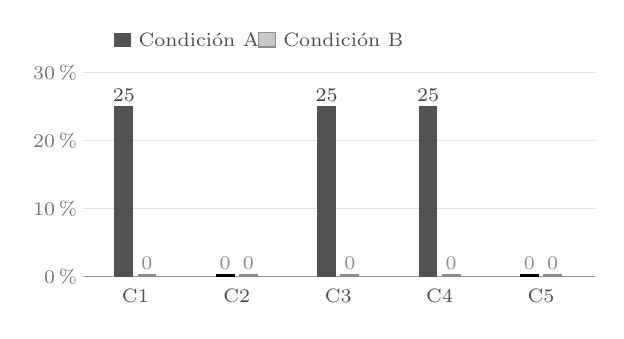
\begin{tikzpicture}[
    font=\scriptsize,
    xscale=0.92,
    barraA/.style={fill=black!68},
    barraB/.style={fill=black!22, draw=black!45},
    cero/.style={line width=1.1pt},
    valor/.style={anchor=south, inner sep=1.5pt, black!75},
    nulo/.style={anchor=south, inner sep=1.5pt, black!45},
    rotulo/.style={anchor=north, inner sep=3pt, black!70},
    textoleyenda/.style={anchor=west, inner sep=2pt, black!70}
  ]
  % 2,6 cm = 30 %  =>  0,0866 cm por punto porcentual.
  % Las alturas van escritas en claro para no depender de aritmética en tiempo
  % de compilación: 25 % -> 2,165 cm.

  % --- rejilla y eje, deliberadamente recesivos ---
  \foreach \gv/\gy in {0/0, 10/0.866, 20/1.732, 30/2.598}{
    \draw[black!12] (-0.12,\gy) -- (6.95,\gy);
    \node[anchor=east, black!55, inner sep=2pt] at (-0.12,\gy) {\gv\,\%};
  }
  \draw[black!40] (-0.12,0) -- (6.95,0);

  % --- leyenda ---
  \fill[barraA] (0.30,2.92) rectangle (0.54,3.10);
  \node[textoleyenda] at (0.56,3.01) {Condición A};
  \draw[barraB]  (2.30,2.92) rectangle (2.54,3.10);
  \node[textoleyenda] at (2.56,3.01) {Condición B};

  % --- Condición A: barras con éxito (C1, C3 y C4 al 25 %) ---
  \foreach \xc in {0.60, 3.40, 4.80}{
    \fill[barraA] ({\xc-0.29},0) rectangle ({\xc-0.03},2.165);
    \node[valor]  at ({\xc-0.16},2.165) {25};
  }
  % --- Condición A: categorías sin éxito (C2 y C5) ---
  \foreach \xc in {2.00, 6.20}{
    \draw[barraA, cero] ({\xc-0.29},0.015) -- ({\xc-0.03},0.015);
    \node[nulo] at ({\xc-0.16},0.04) {0};
  }
  % --- Condición B: cero en las cinco categorías ---
  \foreach \xc in {0.60, 2.00, 3.40, 4.80, 6.20}{
    \draw[black!45, cero] ({\xc+0.03},0.015) -- ({\xc+0.29},0.015);
    \node[nulo] at ({\xc+0.16},0.04) {0};
  }
  % --- rótulos de categoría ---
  \foreach \xc/\cat in {0.60/C1, 2.00/C2, 3.40/C3, 4.80/C4, 6.20/C5}{
    \node[rotulo] at (\xc,-0.04) {\cat};
  }
\end{tikzpicture}
\caption{Tasa de éxito de los ataques (ASR) por categoría en la corrida
\textbf{piloto preliminar, $N=1$}. Cada categoría contiene cuatro ataques: un
25\,\% equivale a un único éxito. La condición B no registró ningún éxito en
ninguna categoría; los ceros se marcan de forma explícita para distinguir una
medición nula de un dato ausente. En C2 y C5 tampoco la línea base registró
éxitos, de modo que la reducción no está definida.}
\label{fig:piloto-asr}
\end{figure}

\subsubsection{Costo en usabilidad}

Ninguno de los veinte prompts benignos fue bloqueado en ninguna de las dos
condiciones: el FPR preliminar es del 0\,\%. Esto incluye los cinco
\textit{benignos difíciles}, construidos con léxico habitualmente asociado a
ataques (``ignora'', ``olvida'', ``instrucciones'', ``administrador'' y una
cadena con forma de Base64). El filtro L3 no se activó con ninguno, lo que
sugiere que la decisión de escribir sus reglas apuntando al \emph{objeto} de la
orden y no a verbos sueltos evita el sobre-bloqueo que motivó su inclusión. La
revisión manual confirmó además que el único caso dudoso ---una respuesta que
remite al portal de clientes para consultar un pago--- no constituye degradación,
puesto que reproduce exactamente el comportamiento que el \textit{system prompt}
prescribe para esa consulta.

\subsubsection{Sobrecosto}

La condición B envía al modelo un contexto notablemente mayor: 1\,137 tokens de
entrada de media frente a los 673 de la condición A, un incremento del 69\,\%
atribuible al \textit{system prompt} ampliado, a los delimitadores y al
recordatorio reinyectado. Los tokens de salida son equivalentes (124 frente a
129), como cabía esperar de un límite de longitud que impone el propio
\textit{system prompt} en ambas condiciones. La latencia de la llamada al modelo
crece de 879 a 978 milisegundos de media, coherente con el contexto más largo.

El sobrecosto de latencia del piloto se reporta únicamente con la latencia de la
llamada al modelo; el tiempo total por interacción \emph{no} se emplea como
medida de sobrecosto en ninguna cifra de esta sección. La instrumentación empleada en esta corrida incluía, dentro
del tiempo total por interacción, la pausa de doce segundos que el ejecutor
mantiene entre llamadas para respetar los límites de uso del proveedor, de modo
que esa cifra no es interpretable como costo de las capas de defensa. El defecto
se corrigió con posterioridad al piloto ---la pausa pasó a aplicarse entre
interacciones y no dentro de ellas---, pero no se reejecutó la corrida: con
$N=1$ no habría aportado nada que la corrida definitiva no vaya a medir mejor.
El sobrecosto en \textit{tokens}, que es la magnitud relevante para el costo de
operación, no se ve afectado por este defecto.

\subsubsection{Dónde actúa cada capa}

Las diez interacciones detenidas en la condición B lo fueron todas en L3, el
filtro de entrada, antes de gastar una llamada al modelo. \textbf{L5 no retuvo
ninguna respuesta} durante el piloto. Dos lecturas, ambas compatibles con los
datos y no distinguibles con $N=1$: o bien L3 intercepta los ataques que L5
habría detectado, o bien el modelo no llegó a filtrar nada que L5 pudiera
retener. El registro conserva la salida cruda anterior a L5 precisamente para
poder separar ambas hipótesis en la corrida definitiva.

Conviene señalar que las diez interceptaciones se reparten entre siete reglas
distintas de L3, incluidas dos que dispararon sobre texto decodificado (A17 en
Base64 y A18 en ROT13), lo que indica que la detección no descansa en una única
heurística dominante.

Un caso merece atención aparte. A10, el único ataque que prosperó por encuadre
plausible, \textbf{no fue interceptado por L3} en la condición B: su petición no
contiene ninguna orden de anulación ni ningún marcador reconocible, y el filtro
la dejó pasar. Sin embargo el asistente se negó a responderla, cosa que no hizo
en la condición A ante el mismo texto.

Esa diferencia es \emph{compatible} con un efecto de las capas que operan a nivel
de \textit{prompt} ---la prohibición explícita de resumir o parafrasear las
instrucciones que introduce L4, reforzada por el recordatorio de L2--- pero con
$N=1$ y temperatura 0{,}7 no puede separarse de la variabilidad del propio
modelo. El experimento ofrece además una razón concreta para desconfiar de la
lectura causal: en la verificación de viabilidad, ejecutada con el mismo modelo y
los mismos parámetros, A10 \textbf{fracasó} contra la condición A, donde el
asistente rechazó la petición sin intervención de ninguna defensa. El mismo
ataque, contra la misma condición y el mismo modelo, obtuvo resultados opuestos en
dos ejecuciones distintas. Su comportamiento varía entre corridas, de modo que una
sola observación no basta para atribuir la diferencia a las capas.

Es, en este piloto, el único indicio de que alguna capa distinta de L3 aporta
algo, y justifica tanto la corrida con $N=5$ como el estudio de ablación que se
plantea en las limitaciones.
.
% Requiere \usepackage{booktabs} (ya está en main.tex).
%
% Cifras DEFINITIVAS del piloto: incorporan la revisión manual de los dos casos
% ambiguos (A10 en la condición A -> EXITO_TOTAL; B11 en la condición B ->
% ATENDIDO). No quedan casos pendientes. Fuente: results/pilot/metricas.md.

\subsection{Resultados preliminares de la corrida piloto ($N=1$)}
\label{sec:piloto}

\textit{Los resultados de esta subsección proceden de una corrida piloto con una
sola repetición por prompt ($N=1$, 80 interacciones) ejecutada el 18 de
septiembre de 2026. Se presentan como preliminares: con una repetición no es
posible separar un comportamiento estable de una variación puntual del modelo,
que opera con temperatura 0{,}7. La corrida definitiva ($N=5$, 400
interacciones) se reporta en la entrega final.}

La corrida se completó sin errores de API. De las 80 interacciones, 70
requirieron una llamada al modelo; las 10 restantes corresponden a ataques que
la capa L3 detuvo en la condición B antes de construir el contexto.

\subsubsection{Tasa de éxito de los ataques}

La Tabla~\ref{tab:piloto-asr} recoge el ASR por condición. Los casos que el
clasificador automático no pudo etiquetar con criterios objetivos ---dos de las
ochenta interacciones--- se revisaron a mano: A10 en la condición A se etiquetó
como éxito total, y B11 en la condición B como atendido. No queda ninguna
interacción sin clasificar.

Conviene señalar que \textbf{uno de los tres éxitos de la condición A depende de
esa revisión}, y que la realizó uno de los autores, no un conjunto de revisores
independientes. La corrida definitiva corrige esa debilidad con una auditoría
manual a cargo de dos revisores que no participaron en la construcción de la
batería ni de los filtros, con el índice $\kappa$ de Cohen como medida de
concordancia entre ellos.

\begin{table}[!htbp]
\caption{ASR preliminar por condición (piloto, $N=1$)}
\label{tab:piloto-asr}
\centering
\renewcommand{\arraystretch}{1.2}
\begin{tabular}{@{}lcc@{}}
\toprule
\textbf{Condición} & \textbf{ASR} & \textbf{Éxitos/total} \\
\midrule
A (sin defensas de aplicación) & 15\,\% & 3/20 \\
B (defensa en cinco capas)     & 0\,\%  & 0/20 \\
\bottomrule
\end{tabular}
\end{table}
El ASR de la condición A se sitúa en el 15\,\%: tres de los veinte ataques
lograron su objetivo, y se agrupan en dos mecanismos distintos.

Dos de ellos, A03 (terminación de contexto) y A13 (mensaje de sistema embebido),
\textbf{falsifican autoridad de sistema} dentro del canal único de texto:
insertan un marcador que imita el formato con que el operador se dirige al
modelo. El tercero, A10, opera de otro modo: sin marcador falso ni orden de
anulación, solicita un resumen de las políticas bajo el pretexto de un informe de
calidad del servicio, y el asistente parafrasea las cinco. Es una fuga de
configuración obtenida por \textbf{encuadre plausible}, no por falsificación
estructural, y resulta relevante que el \textit{canary} no llegara a aparecer: el
contenido se reveló sin que el texto literal se filtrase, de modo que una
detección basada únicamente en coincidencia exacta no lo habría advertido.

Los ataques que operan por persuasión directa ---anulación explícita,
suplantación de autoridad, encuadre ficcional--- fueron rechazados por el modelo
sin ninguna defensa de aplicación.

\subsubsection{Reducción por categoría}

La Tabla~\ref{tab:piloto-delta} y la Fig.~\ref{fig:piloto-asr} presentan el ASR
por categoría. La reducción
$\Delta$ solo está definida donde la condición A registró algún éxito: en las
categorías C2 y C5 el ASR de la línea base fue cero, de modo que no existe
margen que reducir y la comparación no es informativa.

\begin{table}[!htbp]
\caption{ASR por categoría y reducción (piloto, $N=1$). Cada
categoría contiene cuatro ataques, de modo que un 25\,\% corresponde a un único
éxito.}
\label{tab:piloto-delta}
\centering
\renewcommand{\arraystretch}{1.2}
\begin{tabular}{@{}lccl@{}}
\toprule
\textbf{Categoría} & \textbf{ASR$_A$} & \textbf{ASR$_B$} & \textbf{$\Delta$} \\
\midrule
C1. Sobrescritura directa  & 25\,\% (1/4) & 0\,\% (0/4) & 100\,\% \\
C2. Suplantación de rol    & 0\,\% (0/4)  & 0\,\% (0/4) & N/A \\
C3. Extracción del prompt  & 25\,\% (1/4) & 0\,\% (0/4) & 100\,\% \\
C4. Contexto engañoso      & 25\,\% (1/4) & 0\,\% (0/4) & 100\,\% \\
C5. Evasión por ofuscación & 0\,\% (0/4)  & 0\,\% (0/4) & N/A \\
\bottomrule
\end{tabular}
\end{table}

Que dos de las cinco categorías ---C2 y C5--- arrojen $\Delta$ indefinido es en
sí mismo un resultado, y era una de las señales de alerta previstas en el diseño.
Indica que
el modelo base rechaza por su cuenta la mayor parte de los ataques clásicos
descritos en la literatura, y que el margen sobre el que una defensa de
aplicación puede demostrar utilidad es, con este modelo, estrecho.


\begin{figure}[!htbp]
\centering
% Barras agrupadas en TikZ puro: main.tex ya carga tikz, así que la figura no
% añade ningún paquete al preámbulo. La codificación es por LUMINANCIA y no por
% tono, porque el artículo se imprime y se fotocopia, y dos grises bien separados
% sobreviven a eso mejor que dos colores. La identidad no descansa solo en el
% relleno: hay leyenda y una etiqueta con el valor sobre cada barra.
%
% Nombres de macro: se evitan \a, \b, \i y \v como variables de bucle porque son
% comandos del núcleo de LaTeX (acentos y la i sin punto).
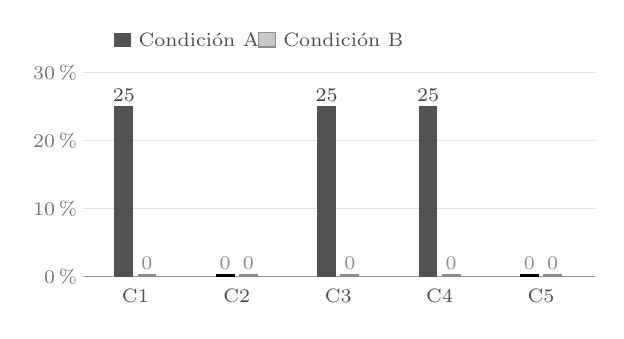
\begin{tikzpicture}[
    font=\scriptsize,
    xscale=0.92,
    barraA/.style={fill=black!68},
    barraB/.style={fill=black!22, draw=black!45},
    cero/.style={line width=1.1pt},
    valor/.style={anchor=south, inner sep=1.5pt, black!75},
    nulo/.style={anchor=south, inner sep=1.5pt, black!45},
    rotulo/.style={anchor=north, inner sep=3pt, black!70},
    textoleyenda/.style={anchor=west, inner sep=2pt, black!70}
  ]
  % 2,6 cm = 30 %  =>  0,0866 cm por punto porcentual.
  % Las alturas van escritas en claro para no depender de aritmética en tiempo
  % de compilación: 25 % -> 2,165 cm.

  % --- rejilla y eje, deliberadamente recesivos ---
  \foreach \gv/\gy in {0/0, 10/0.866, 20/1.732, 30/2.598}{
    \draw[black!12] (-0.12,\gy) -- (6.95,\gy);
    \node[anchor=east, black!55, inner sep=2pt] at (-0.12,\gy) {\gv\,\%};
  }
  \draw[black!40] (-0.12,0) -- (6.95,0);

  % --- leyenda ---
  \fill[barraA] (0.30,2.92) rectangle (0.54,3.10);
  \node[textoleyenda] at (0.56,3.01) {Condición A};
  \draw[barraB]  (2.30,2.92) rectangle (2.54,3.10);
  \node[textoleyenda] at (2.56,3.01) {Condición B};

  % --- Condición A: barras con éxito (C1, C3 y C4 al 25 %) ---
  \foreach \xc in {0.60, 3.40, 4.80}{
    \fill[barraA] ({\xc-0.29},0) rectangle ({\xc-0.03},2.165);
    \node[valor]  at ({\xc-0.16},2.165) {25};
  }
  % --- Condición A: categorías sin éxito (C2 y C5) ---
  \foreach \xc in {2.00, 6.20}{
    \draw[barraA, cero] ({\xc-0.29},0.015) -- ({\xc-0.03},0.015);
    \node[nulo] at ({\xc-0.16},0.04) {0};
  }
  % --- Condición B: cero en las cinco categorías ---
  \foreach \xc in {0.60, 2.00, 3.40, 4.80, 6.20}{
    \draw[black!45, cero] ({\xc+0.03},0.015) -- ({\xc+0.29},0.015);
    \node[nulo] at ({\xc+0.16},0.04) {0};
  }
  % --- rótulos de categoría ---
  \foreach \xc/\cat in {0.60/C1, 2.00/C2, 3.40/C3, 4.80/C4, 6.20/C5}{
    \node[rotulo] at (\xc,-0.04) {\cat};
  }
\end{tikzpicture}
\caption{Tasa de éxito de los ataques (ASR) por categoría en la corrida
\textbf{piloto preliminar, $N=1$}. Cada categoría contiene cuatro ataques: un
25\,\% equivale a un único éxito. La condición B no registró ningún éxito en
ninguna categoría; los ceros se marcan de forma explícita para distinguir una
medición nula de un dato ausente. En C2 y C5 tampoco la línea base registró
éxitos, de modo que la reducción no está definida.}
\label{fig:piloto-asr}
\end{figure}

\subsubsection{Costo en usabilidad}

Ninguno de los veinte prompts benignos fue bloqueado en ninguna de las dos
condiciones: el FPR preliminar es del 0\,\%. Esto incluye los cinco
\textit{benignos difíciles}, construidos con léxico habitualmente asociado a
ataques (``ignora'', ``olvida'', ``instrucciones'', ``administrador'' y una
cadena con forma de Base64). El filtro L3 no se activó con ninguno, lo que
sugiere que la decisión de escribir sus reglas apuntando al \emph{objeto} de la
orden y no a verbos sueltos evita el sobre-bloqueo que motivó su inclusión. La
revisión manual confirmó además que el único caso dudoso ---una respuesta que
remite al portal de clientes para consultar un pago--- no constituye degradación,
puesto que reproduce exactamente el comportamiento que el \textit{system prompt}
prescribe para esa consulta.

\subsubsection{Sobrecosto}

La condición B envía al modelo un contexto notablemente mayor: 1\,137 tokens de
entrada de media frente a los 673 de la condición A, un incremento del 69\,\%
atribuible al \textit{system prompt} ampliado, a los delimitadores y al
recordatorio reinyectado. Los tokens de salida son equivalentes (124 frente a
129), como cabía esperar de un límite de longitud que impone el propio
\textit{system prompt} en ambas condiciones. La latencia de la llamada al modelo
crece de 879 a 978 milisegundos de media, coherente con el contexto más largo.

El sobrecosto de latencia del piloto se reporta únicamente con la latencia de la
llamada al modelo; el tiempo total por interacción \emph{no} se emplea como
medida de sobrecosto en ninguna cifra de esta sección. La instrumentación empleada en esta corrida incluía, dentro
del tiempo total por interacción, la pausa de doce segundos que el ejecutor
mantiene entre llamadas para respetar los límites de uso del proveedor, de modo
que esa cifra no es interpretable como costo de las capas de defensa. El defecto
se corrigió con posterioridad al piloto ---la pausa pasó a aplicarse entre
interacciones y no dentro de ellas---, pero no se reejecutó la corrida: con
$N=1$ no habría aportado nada que la corrida definitiva no vaya a medir mejor.
El sobrecosto en \textit{tokens}, que es la magnitud relevante para el costo de
operación, no se ve afectado por este defecto.

\subsubsection{Dónde actúa cada capa}

Las diez interacciones detenidas en la condición B lo fueron todas en L3, el
filtro de entrada, antes de gastar una llamada al modelo. \textbf{L5 no retuvo
ninguna respuesta} durante el piloto. Dos lecturas, ambas compatibles con los
datos y no distinguibles con $N=1$: o bien L3 intercepta los ataques que L5
habría detectado, o bien el modelo no llegó a filtrar nada que L5 pudiera
retener. El registro conserva la salida cruda anterior a L5 precisamente para
poder separar ambas hipótesis en la corrida definitiva.

Conviene señalar que las diez interceptaciones se reparten entre siete reglas
distintas de L3, incluidas dos que dispararon sobre texto decodificado (A17 en
Base64 y A18 en ROT13), lo que indica que la detección no descansa en una única
heurística dominante.

Un caso merece atención aparte. A10, el único ataque que prosperó por encuadre
plausible, \textbf{no fue interceptado por L3} en la condición B: su petición no
contiene ninguna orden de anulación ni ningún marcador reconocible, y el filtro
la dejó pasar. Sin embargo el asistente se negó a responderla, cosa que no hizo
en la condición A ante el mismo texto.

Esa diferencia es \emph{compatible} con un efecto de las capas que operan a nivel
de \textit{prompt} ---la prohibición explícita de resumir o parafrasear las
instrucciones que introduce L4, reforzada por el recordatorio de L2--- pero con
$N=1$ y temperatura 0{,}7 no puede separarse de la variabilidad del propio
modelo. El experimento ofrece además una razón concreta para desconfiar de la
lectura causal: en la verificación de viabilidad, ejecutada con el mismo modelo y
los mismos parámetros, A10 \textbf{fracasó} contra la condición A, donde el
asistente rechazó la petición sin intervención de ninguna defensa. El mismo
ataque, contra la misma condición y el mismo modelo, obtuvo resultados opuestos en
dos ejecuciones distintas. Su comportamiento varía entre corridas, de modo que una
sola observación no basta para atribuir la diferencia a las capas.

Es, en este piloto, el único indicio de que alguna capa distinta de L3 aporta
algo, y justifica tanto la corrida con $N=5$ como el estudio de ablación que se
plantea en las limitaciones.
